\documentclass[10pt]{beamer}

\usepackage[UKenglish]{babel}
\usepackage{hyperref}
\usepackage[utf8]{inputenc}
\usepackage[backend=bibtex,style=ieee,maxbibnames=99]{biblatex}
\usepackage[uni,footuni,headframelogo]{./unirostock/beamerthemeRostock}
\usepackage{scrhack} %Fix for older packages

\title{IuK-Blockchain}
\subtitle{Progress report}
\author{\textsc{Robert Kohlen}\newline\textsc{Richard Dabels}\newline\textsc{Maximilian Jung}\newline\textsc{Daniel Decker}\newline\textsc{Nis Meinert}\newline\textsc{Hannes Hagen}}
\date{03.06.2018}
\footinstitute{Institut für Informatik}

\addbibresource{./references.bib}

\begin{document}

\begin{frame}
	\titlepage
\end{frame}

\begin{frame}{Task}
	\begin{itemize}
		\item Develop a private blockchain to use at the IuK chair
		\item Implement an example scenario to:
		\begin{itemize}
			\item Verify the autenticity of documents with the help of blockchains
			\item A way to add documents or hashes of documents to the blockchain
		\end{itemize}
	\end{itemize}
\end{frame}

\begin{frame}{Progress}
	\begin{itemize}
		\item Framework: Parity (Etherum)
		\item Web interface: Mostly implemented
	\end{itemize}
\end{frame}

\begin{frame}{Parity}
	\begin{itemize}
		\item Implementation of the Etherum blockchain
		\item Supports Proof of Authority (PoA)
		\begin{itemize}
			\item Blocks can only be added by approved accounts
		\end{itemize}
		\item Developed by 131 contributors on GitHub
	\end{itemize}
\end{frame}

\begin{frame}{Contract}
	\begin{itemize}
		\item Storing documents as hashes
		\item Setting authors for documents
		\item Enabling revision of old documents
		\item Enabling revocation of documents
		\item Still unsure about some topics ... (later)
	\end{itemize}
\end{frame}

\begin{frame}{Docker}
	\begin{itemize}
		\item Running nodes in Docker
		\item Parity deploy script to generate deployment configurations
	\end{itemize}
\end{frame}

\begin{frame}{Web interface}
	\begin{itemize}
		\item Mostly functional
		\item Not yet working on our blockchain
		\item Uses Metamask to interact with the blockchain
	\end{itemize}
\end{frame}

\begin{frame}{Web interface}
	\begin{figure}
		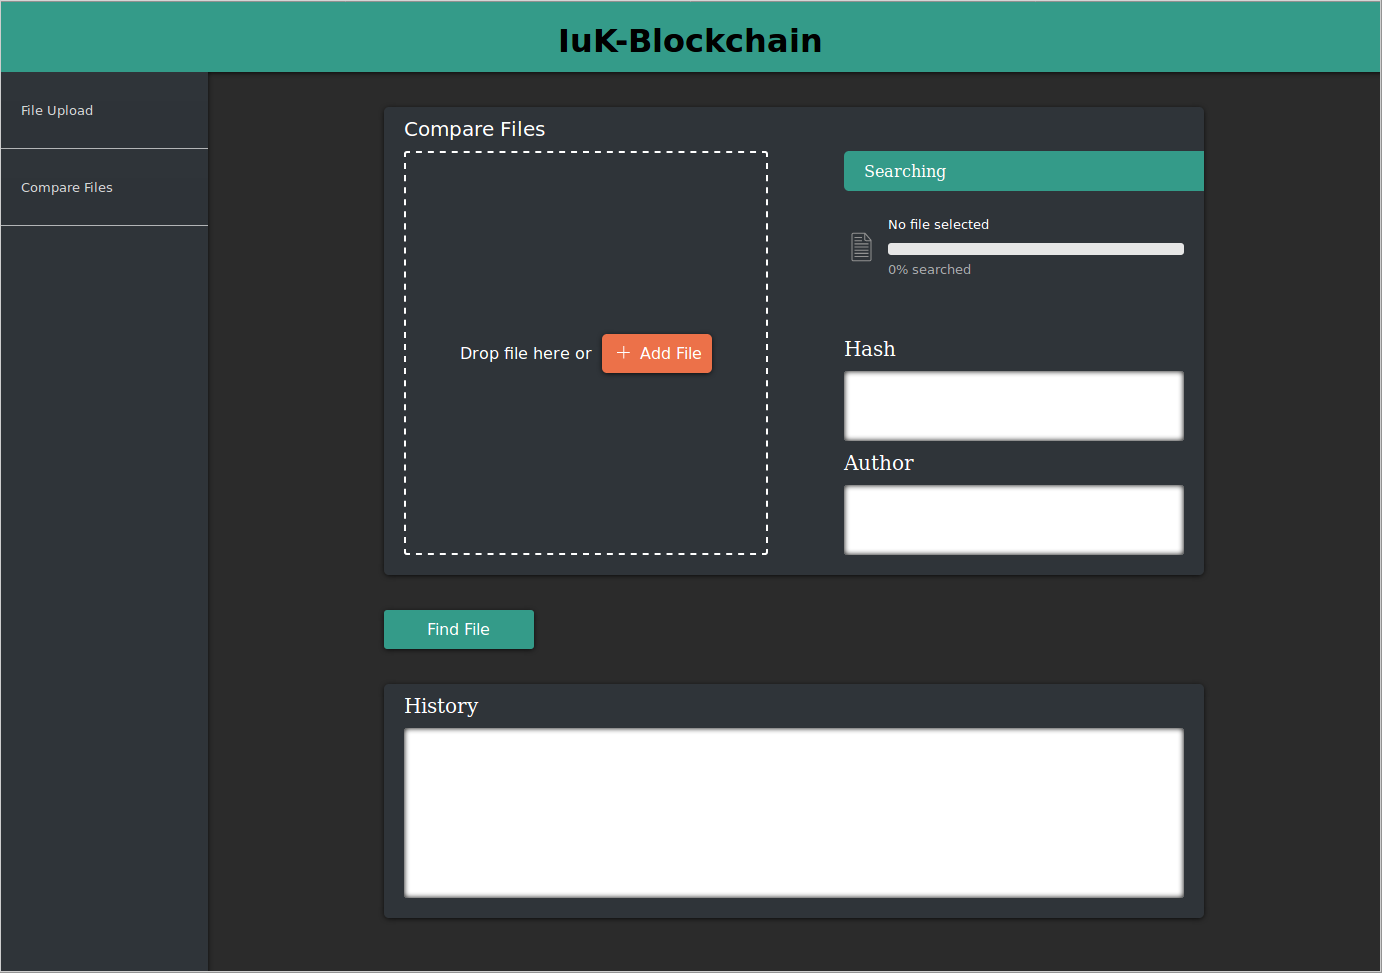
\includegraphics[width=1\textwidth]{images/GUI-180603_1.png}
	\end{figure}
\end{frame}

\begin{frame}{Open questions}
	\begin{itemize}
		\item Should ownership of an document be changable?
		\item Are fees/transaction-gas necessary to prevent spam?
	\end{itemize}
\end{frame}

%\begin{frame}[allowframebreaks]{References}
%Reduce URL font size
%\renewcommand{\UrlFont}{\small\rmfamily}
%\printbibliography
%\end{frame}

\end{document}
